% !TEX encoding = UTF-8
% !TEX TS-program = pdflatex
% !TEX root = ../tesi.tex

%**************************************************************
\chapter{Resoconto Stage}
\label{cap:resoconto-stage}
%**************************************************************

%**************************************************************
\section{Pianificazione}
\subsection{Pianificazione iniziale}\label{sec:pianificazione-iniziale}
Una prima pianificazione delle attività è stata fatta da me insieme al tutor aziendale, prima dell'inizio dello stage, principalmente definendo il Piano di Lavoro, documento necessario per iniziare lo stage e per avere un'idea delle tempistiche necessarie al completamento degli obiettivi discussi. Durante lo svolgimento dello stage tuttavia, la pianificazione originaria ha subito delle piccole modifiche, in quanto alcune attività hanno richiesto più tempo di altre. 

\subsection{Sistema di Issue e Gantt}
Per essere sempre entrambi aggiornati sullo stato dei lavori, il mio tutor mi ha suggerito di utilizzare il sistema di Issue ampiamente utilizzato in azienda basato su Redmine, abbiamo quindi riportato gli obiettivi principali definiti nel Piano di Lavoro, in modo da tenere traccia degli obiettivi completati e di una stima del tempo richiesto, è possibile infatti segnare una stima delle ore utilizzate per una certa attività. Redmine era inoltre collegato con il git aziendale, permettendo quindi di fare riferimento a specifici commit e di scrivere una Wiki relativa al progetto.
\\
Impostando correttamente le date e le priorità tra le attività da svolgere nel Redmine aziendale, era anche possibile generare automaticamente un diagramma Gantt per visualizzare in maniera più semplice lo stato delle attività, le scadenze e i tempi di ogni attività per capire se è in ritardo o in anticipo. Questo essendo un progetto relativamente piccolo è stato utilizzato poco, ma è stato molto utile per imparare come viene gestito un progetto più ampio in azienda.

\subsection{Discussioni e incontri con il tutor}
Discutere con il tutor e aggiornarlo sullo stato del progetto e su eventuali dubbi/problemi è stata una parte fondamentale del mio stage, soprattutto lavorando principalmente da casa. Per questo facevamo una videochiamata al giorno (quando possibile) per discutere lo stato e i prossimi passi da fare. Inoltre ci incontravamo di persona in ufficio almeno una o due volte a settimana, principalmente per mostrargli lo stato dei lavori e fare delle piccole dimostrazioni su cosa era stato fatto e in che modo, ma anche per discutere su come migliorare alcuni dettagli o come risolvere alcuni problemi.

\subsection{Problemi e ritardi}
Come accennato nella sezione \nameref{sec:pianificazione-iniziale} e come vedremo più nel dettaglio tra poco, la pianificazione iniziale ha subito delle piccole modifiche, in quanto alcune attività hanno richiesto più tempo. Questo non è stato un grosso problema perché, viceversa, alcune attività hanno richiesto meno tempo. I problemi principali sono stati nell'utilizzo di CMake e nell'import di un volume attraverso le librerie aziendali.

%**************************************************************
\section{Implementazione}
\subsection{Impostazione ambiente di sviluppo}
La prima settimana era dedicata all'introduzione del progetto, dovevo quindi impostare l'ambiente di sviluppo, discutere con il tutor le modalità di lavoro, gli strumenti, configurare il git aziendale e studiare le librerie che avrei utilizzato, tutti passi preliminari e necessari ad un corretto svolgimento dello stage.
Dopo aver impostato tutti gli strumenti, come Visual Studio con il compilatore corretto, aver installato l'ultima versione di Qt e di QtCreator, il primo passo è stato scaricare e studiare le librerie che sarebbero state utilizzate, quindi principalmente VTK, con uno studio preliminare di 3D Slicer per imparare le basi di come viene utilizzato il Volume Rendering, come importare un volume DICOM e dettagli simili. 

\subsection{Studio di 3D Slicer}
Per analizzare al meglio il funzionamento di 3D Slicer, ad inizio stage si era pensato di compilarlo dai sorgenti in modo da poterne effettuare il debug, tuttavia si è rivelato un processo molto arduo, in quanto la documentazione su come compilarlo non era molto precisa, e fare una build con quasi tutti i moduli ha richiesto anche più di 6 ore su un processore Intel i7 6700k composto da 4 core/8 thread a 4.2Ghz. Dopo qualche tentativo fallito quindi, l'idea è stata abbandonata in quanto non strettamente necessaria. 3D Slicer è stato quindi installato normalmente dal setup disponibile nel sito, ed il suo sorgente è stato sfogliato principalmente attraverso GitHub.

\subsection{Studio e installazione di VTK}
Anche VTK, come ogni libreria, ha pro e contro: un contro che purtroppo ho notato subito è che c'è della documentazione molto aggiornata e altra molto datata. Per esempio, cercando su Google:"How to build vtk", uno dei primi risultati è: \href{https://vtk.org/Wiki/VTK/Building/Windows}{vtk.org/Wiki/VTK/Building/Windows}, pagina con ultimo aggiornamento al 2014 nel momento in cui questo documento è stato scritto. \'E comunque una documentazione valida per le basi, ma è chiaro che non può essere utilizzata attivamente. Discretamente meglio è la pagina \href{https://vtk.org/Wiki/VTK/Configure_and_Build}{vtk.org/Wiki/VTK/Configure\_and\_Build} , aggiornata al 2017. Avendo già effettuato altri progetti e compilazioni con CMake, non ho avuto grossa difficoltà a compilare VTK comunque, in quanto è davvero ben gestita e facile da configurare. CMake può essere utilizzato normalmente da linea di comando o da interfaccia grafica tramite CMake-gui, installato insieme a CMake. Per una libreria di queste dimensioni con molte proprietà da configurare, è molto più comodo utilizzare la gui che permette di visualizzare lo stato di tutte le variabili prima di generare il progetto da compilare.

\begin{figure}[h]
    \centering
    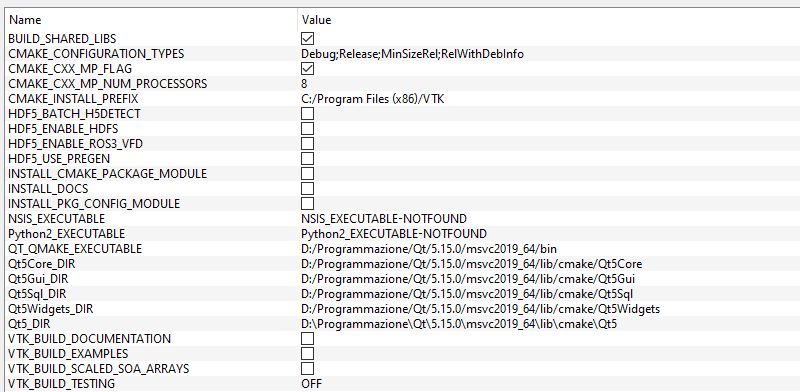
\includegraphics[width=1\textwidth]{immagini/svolgimento/vtkcmake.png}
    \caption{\textit{Alcuni parametri di configurazione di VTK su CMake-gui}}
    \textbf{Fonte}: Stage
    \label{fig: VTK CMAKE}
\end{figure}

A parte qualche dubbio nella compilazione tuttavia, VTK offre una ampia gamma di esempi, ed è stato quindi molto interessante ed utile analizzarne i principali per comprenderne il funzionamento e le basi. Oltre agli esempi ufficiali comunque, se ne trovano moltissimi anche su GitHub, grazie alla comunità.

\subsection{Primo CMakeLists}
Come menzionato nella sezione precedente, avevo esperienza nel fare la compilazione di alcune librerie utilizzando CMake, ma non lo avevo mai utilizzato in un progetto personale. Nel Piano di Lavoro CMake era segnato come obiettivo facoltativo con:"F03: porting librerie aziendali su CMake;". \'E stato invece deciso con il tutor di iniziare il progetto direttamente utilizzando CMake: innanzitutto per imparare come utilizzarlo e le basi, ma anche per non dover cambiare sistema di build in seguito.
\\
Qt utilizza di default un sistema di build basato su Makefile, generati tramite il comando proprietario qmake su un progetto ".pro". Questo funziona molto bene con Qt ma è specifico per l'utilizzo con Qt, CMake è un sistema di build molto più generico e ampiamente utilizzato. L'azienda voleva esplorarne le capacità e le funzionalità, e anche io ero molto interessato ad imparare come utilizzarlo meglio. CMake funziona tramite la scrittura di uno o più CMakeLists.txt, che definiscono tutti i parametri di configurazione del progetto, le librerie esterne, e i file da compilare. Per nostra fortuna Qt ha il supporto a CMake quindi non è complesso da integrare. Diamo un'occhiata ad un semplice CMakeLists.txt di base per Qt.

\begin{minted}
[
frame=lines,
fontsize=\footnotesize,
linenos
]{cmake}
cmake_minimum_required(VERSION 3.15.4)

project(helloworld)

set(CMAKE_AUTOMOC ON)
set(CMAKE_AUTORCC ON)

find_package(Qt5 COMPONENTS Widgets REQUIRED)

add_executable(helloworld
    mainwindow.ui
    mainwindow.cpp
    main.cpp
    resources.qrc
)

target_link_libraries(helloworld Qt5::Widgets)
\end{minted}

Analizziamolo per comprenderne i punti principali:
\begin{itemize}
	\item cmake\_minimum\_required: definisce la versione minima di CMake richiesta dal progetto;
	\item project: definisce il nome del progetto e di conseguenza tutte le variabili relative (come per esempio PROJECT\_SOURCE\_DIR);
	\item set imposta una variabile ad un certo valore, nel nostro caso le variabili CMAKE\_AUTOMOC e CMAKE\_AUTORCC sono variabili utilizzate da Qt per specificare di usare il moc e la gestione dei file di risorse;
	\item find\_package: definisce una libreria da trovare ed utilizzare. In caso la posizione di tale libreria non sia nota (per esempio in una variabile di sistema) bisogna passare a CMake il percorso, con una variabile che nel caso di Qt sarà Qt5\_DIR;
	\item add\_executable: definisce l'eseguibile da creare con la relativa lista di file da compilare. Notare che non ci sono i file .h che di norma vengono letti automaticamente, salvo casi particolari;
	\item target\_link\_libraries: definisce le librerie di cui fare il linking nell'eseguibile.
\end{itemize}

\subsection{Ripasso Qt}
Comprese le basi di CMake, dovevo ripassare le funzionalità e la struttura di Qt: avendolo già utilizzato per il progetto di Programmazione ad Oggetti, lo conoscevo già abbastanza bene. Tuttavia dovevo discutere con l'azienda che tipo di interfaccia fare, come strutturare le classi dei widget e come gestire i segnali di click dei tasti. Ho dovuto quindi progettare e realizzare l'interfaccia di base che sarebbe poi stata utilizzata.

\subsection{Integrazione Qt-VTK}
Come accennato nella sezione \nameref{sec:qt-integrazione}, VTK è stato compilato con il supporto a Qt. Questo offre classi come QVTKOpenGLNativeWidget, da cui è possibile derivare un Widget Qt. Un punto molto importante discusso con il tutor aziendale, è stato fare sin da subito in modo che il widget Qt derivato da QVTKOpenGLNativeWidget, che d'ora in poi chiameremo RenderWidget, fosse indipendente: questo per permettere che fosse facilmente trasferibile ad altre applicazioni, con il minor numero possibile di dipendenze, questo si può vedere nella figura \ref{fig: basicwidget}.
\\
Per testare la funzionalità del primo RenderWidget, ho cercato degli esempi su GitHub che mostrassero come caricare un semplice modello 3D su VTK, in modo da assicurarmi che la base funzionasse prima di passare al caricamento di un volume vero e proprio.

\subsection{Volume Mapper}
Come accennato nella sezione \nameref{sec:oggetti-rendering} e in particolare in \nameref{sec:special-rendering}, un oggetto va visualizzato tramite un vtkMapper. Nel caso del Volume Rendering, questo può essere fatto utilizzando vtkGPUVolumeRayCastMapper, un mapper che effettua il ray casting sfruttando l'accelerazione hardware della GPU. Questo è il mapper principale che è stato utilizzato, tuttavia in alcuni casi potrebbe non essere disponibile una GPU, è stato quindi deciso di far controllare all'applicazione se è disponibile una GPU sopportata, in caso contrario utilizzerà invece un vtkSmartVolumeMapper, un mapper "intelligente" che supporta varie modalità: di default utilizzerà una GPU se disponibile, altrimenti passerà automaticamente a vtkFixedPointRayCastMapper , un ray caster software che chiaramente è notevolmente più lento.

\subsection{Primo prototipo}
Una volta creato e testato il RenderWidget, il primo prototipo di visualizzatore volumetrico è stato fatto caricando le immagini con il loader di VTK, chiamato vtkDICOMImageReader. \'E sufficiente infatti indicargli la cartella da leggere perché provi automaticamente a caricare il volume contenuto in tale cartella, il risultato si può vedere nell'immagine \ref{fig: firstvolume}. Notare che molti esami TC e RM potrebbero registrare tutte le immagini (e quindi i volumi) in un'unica cartella. In questo caso non è possibile utilizzare vtkDICOMImageReader, che con le impostazioni di default cerca invece di caricare un singolo volume da tutti i file presenti nella cartella. Nel caso fossero tutti raggruppati in un'unica cartella, i volumi si possono separare con vari programmi, in ogni caso il primo esame DICOM fornitomi dall'azienda era già un singolo volume in una singola cartella, di conseguenza molto semplice da gestire.

\begin{figure}[h]
    \centering
    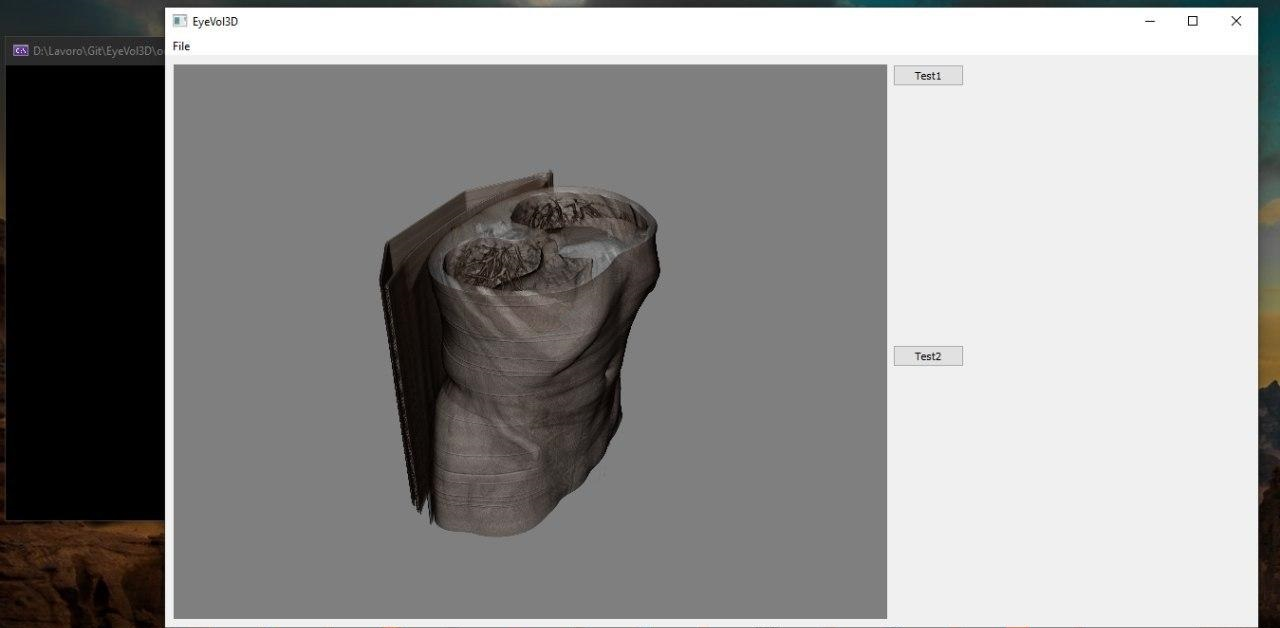
\includegraphics[width=1\textwidth]{immagini/svolgimento/firstvolume.jpg}
    \caption{\textit{Primo Volume Rendering}}
    \textbf{Fonte}: Stage
    \label{fig: firstvolume}
\end{figure}

\subsection{Strumenti di base - Rotazione}
Ottenuto il primo Volume Rendering, una delle prime cose essenziali era la possibilità di ruotarlo/farne lo zoom e interazioni di base simili. Per nostra fortuna VTK fornisce vtkRenderWindowInteractor che consente di definire un'interazione con la nostra finestra di rendering. Nel nostro caso volevamo una camera che ci consentisse di ruotare attorno al volume utilizzando il mouse, in VTK è chiamata vtkInteractorStyleTrackballCamera. \'E bastato quindi creare un vtkRenderWindowInteractor ed indicargli la finestra di rendering da utilizzare, e assegnargli un'interazione di tipo vtkInteractorStyleTrackballCamera per ottenere il risultato desiderato.

\subsection{Strumenti di base - Preset}
A questo punto, è stato il momento di aggiungerci i primi strumenti necessari a modificare e meglio visualizzare il volume: il primo e più importante è stato aggiungere la lista di Preset, una lista predefinita e standard di funzioni di trasferimento. Come accennato in precedenza, questa è stata presa dal repository di 3D Slicer controllando e rispettandone la licenza. Tuttavia questa lista era in XML, e con un XML ci si fa poco, visto che le funzioni di trasferimento vanno inserite in VTK tramite appositi oggetti. Ho deciso quindi insieme al tutor di fare una piccola libreria designata solo a caricare questo XML correttamente in VTK, chiamandola PresetParser. Questa libreria carica l'XML di preset e riempie un array di oggetti generici chiamati VolumePropertyEntry con tutte le proprietà, sarà poi all'applicazione utilizzare questi valori, nel nostro caso caricandoli su VTK. Questo nel mio programma viene fatto all'avvio, caricando la lista dei preset e visualizzando i nomi disponibili. I valori effettivi vengono caricati in VTK solo quando questo è selezionato, visto che comunque sono pochi e non è un'operazione complessa.
\\
Selezionato un preset quindi, Qt esegue il segnale di "cambio selezione" ed esegue la relativa funzione, che nel mio caso legge la entry del preset e crea gli oggetti di VTK vtkVolumeProperty/vtkPiecewiseFunction/vtkColorTransferFunction, impostandoli poi per il volume corrente.

\subsection{Strumenti di base - Mark}
Mark è il nome che la mia azienda ha dato ad un piccolo omino stilizzato, già utilizzato in alcune loro applicazioni. Mark è molto utile in un contesto tridimensionale, in cui è necessario comprendere l'orientamento di ciò che si sta osservando: immaginate di guardare la TC di una gamba, senza un indicatore di com'è orientata la gamba, ci si potrebbe confondere sul sopra/sotto. Come ogni oggetto che viene visualizzato, Mark di base è un vtkActor, di cui è fatto il render tramite un oggetto vtkDataSetMapper. Essendo un'usanza comune avere un widget che mostra l'orientamento, vtk offre l'oggetto apposito vtkOrientationMarkerWidget, a cui noi assegneremo il nostro vtkActor contenente la mesh di Mark. Una volta caricato si può posizionare in un angolo della finestra e abilitare in maniera simile a come fatto per la vtkInteractorStyleTrackballCamera, il risultato è visibile nella figura \ref{fig: basicwidget}.

\subsection{Strumenti di base - MIP e Smoothing}
Un altro punto molto importante è consentire la possibilità di visualizzare la MIP, questo è stato facile da implementare in quanto VTK offre già dei flag per cambiare modalità, come possiamo vedere nell'esempio sottostante:
\begin{minted}
[
frame=lines,
fontsize=\footnotesize
]{cpp}
//Max Intensity Proj
setMapperBlendMode(vtkVolumeMapper::MAXIMUM_INTENSITY_BLEND);
//Min Intensity Proj
setMapperBlendMode(vtkVolumeMapper::MINIMUM_INTENSITY_BLEND);
//Default composite
setMapperBlendMode(vtkVolumeMapper::COMPOSITE_BLEND);
\end{minted}

Come si può notare è presete anche la Minimum Intensity, che raramente è utilizzata, ma è stata inserita comunque sotto consiglio del tutor. Com'è intuibile dal nome, funziona come la MIP ma utilizzando i valori minimi incontrati lungo il raggio. Nel caso fosse necessario, è immediato aggiungere anche la AVERAGE\_INTENSITY\_BLEND.

Lo Smoothing, chiamato anche Jittering, è una funzione che aggiunge un noise alla texture, cercando di rimuovere o ridurre l'effetto di "venatura del legno"(wood-grain effect). Si può notare la differenza nell'immagine \ref{fig: firstvolume}, soprattutto appena sotto il naso. Notare che questa funzione è disponibile solo nel vtkGPUVolumeRayCastMapper, non è infatti disponibile utilizzando il mapper software.

\begin{figure}[h]
    \centering
    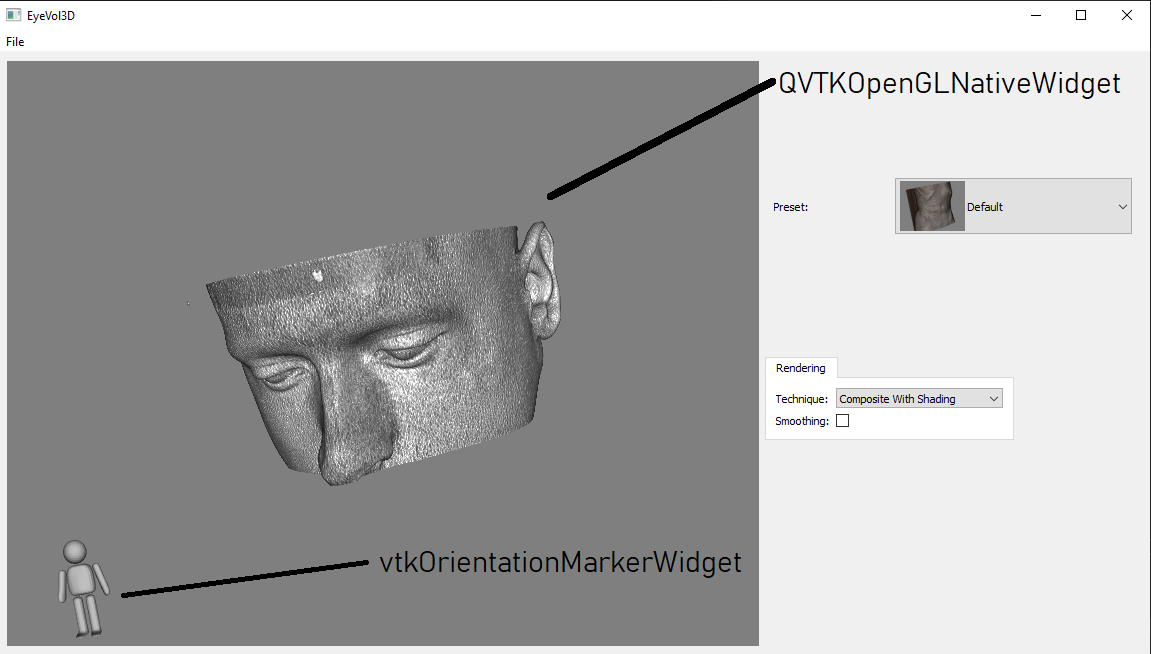
\includegraphics[width=1\textwidth]{immagini/svolgimento/basicwidget.png}
    \caption{\textit{Prima interfaccia con strumenti}}
    \textbf{Fonte}: Stage
    \label{fig: basicwidget}
\end{figure}

\begin{figure}[h]
    \centering
    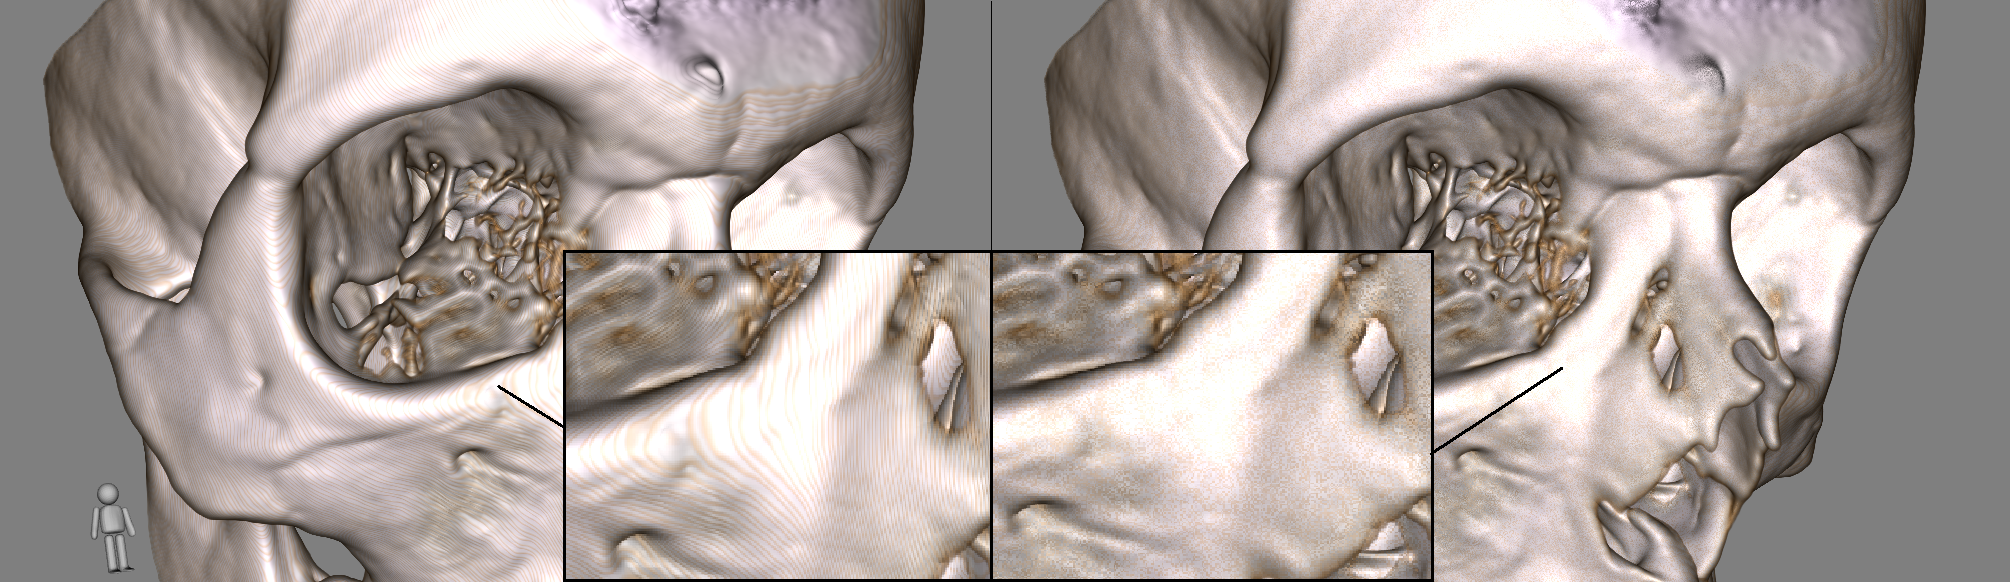
\includegraphics[width=1\textwidth]{immagini/svolgimento/smoothing.png}
    \caption{\textit{Esempio di Smoothing su GPU, OFF a sinistra ed ON a destra}}
    \textbf{Fonte}: Stage
    \label{fig: firstvolume}
\end{figure}

\subsection{Strumenti aggiuntivi - Funzione Threshold}

\subsection{Strumenti aggiuntivi - Taglio tramite box}
\begin{figure}[h]
    \centering
    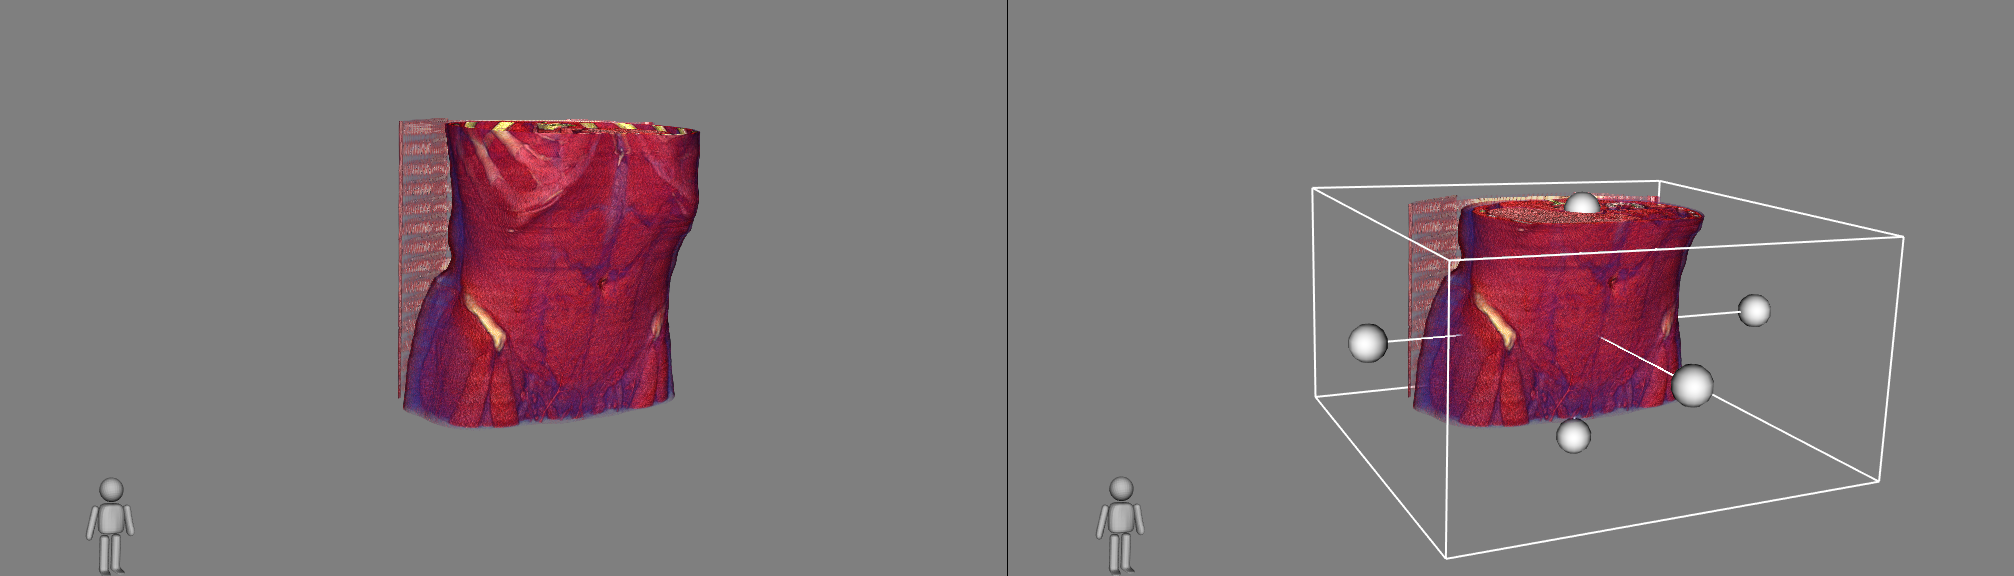
\includegraphics[width=1\textwidth]{immagini/svolgimento/boxcrop.png}
    \caption{\textit{Esempio di taglio del volume tramite vtkBoxWidget}}
    \textbf{Fonte}: Stage
    \label{fig: Taglio Box}
\end{figure}

\subsection{Strumenti aggiuntivi - Taglio tramite plane}
\begin{figure}[h]
    \centering
    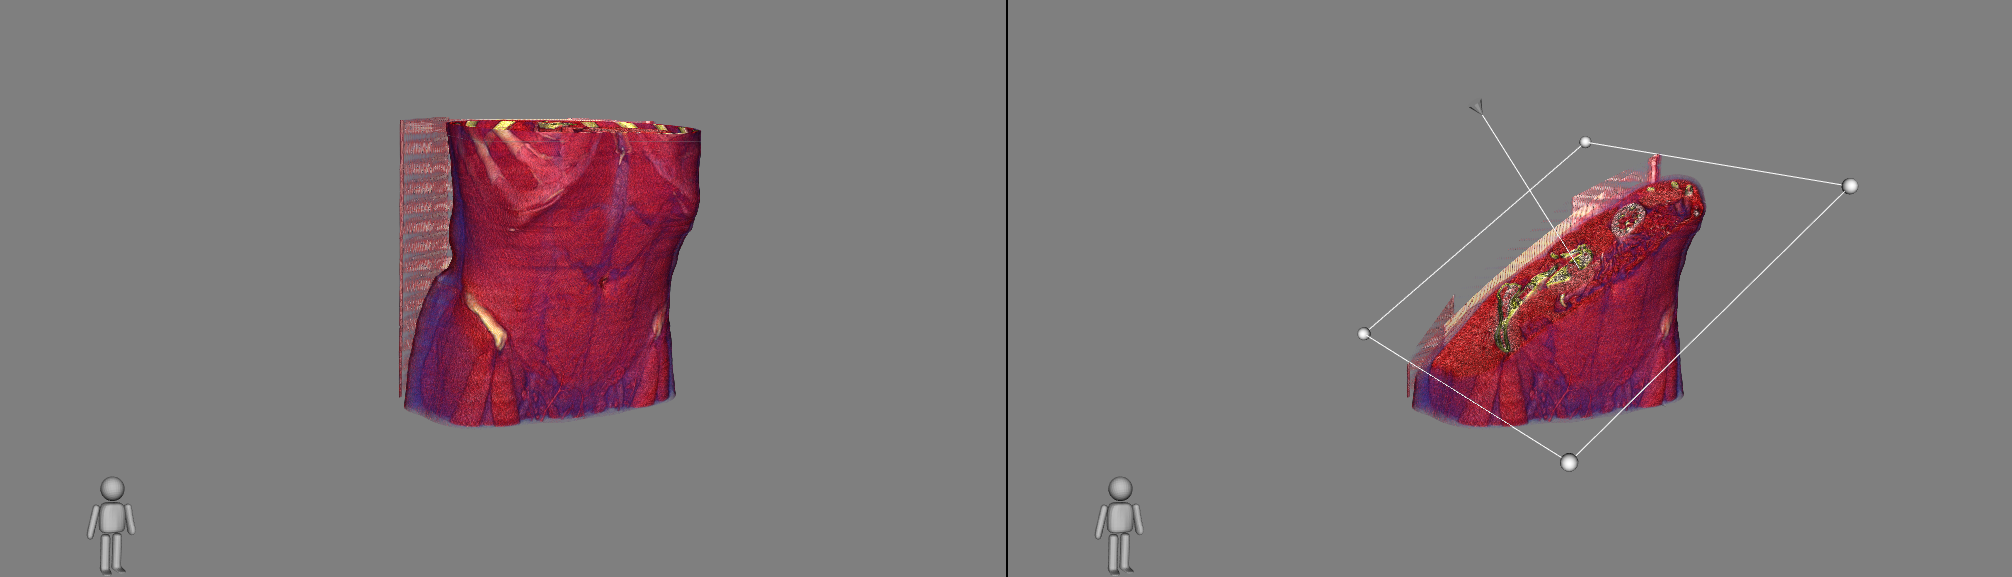
\includegraphics[width=1\textwidth]{immagini/svolgimento/planecrop.png}
    \caption{\textit{Esempio di taglio del volume tramite vtkPlaneWidget}}
    \textbf{Fonte}: Stage
    \label{fig: Taglio Plane}
\end{figure}

\subsection{Compilazione librerie aziendali}
\intro{Le librerie aziendali da utilizzare e i problemi nel compilarle}\\

\subsection{Problemi librerie aziendali}
\intro{I problemi nell'utilizzare le librerie aziendali con VTK}\\

\subsection{Modifiche interfaccia}
\intro{Com'è stata modificata l'interfaccia per renderla semplice e portatile}\\

%**************************************************************
\section{Documentazione}

%**************************************************************
\section{Test}
\subsection{Possibili test su una UI}
\intro{I problemi nel testare un'interfaccia grafica}\\

\subsection{Test di 3D Slicer e VTK}
\intro{Come 3D Slicer e VTK fanno questi test}\\

\subsection{Test implementati}
\intro{Discussione sui test fatti su librerie statiche e "model"}\\